\documentclass[a4paper,12pt]{article}
\usepackage[russian, english]{babel}

\babelfont{rm}{Times New Roman}
\babelfont{sf}{Times New Roman}

\usepackage[hidelinks]{hyperref}
\usepackage{indentfirst}
\usepackage{listings}
\usepackage{xcolor}
\usepackage{here}
\usepackage{array}
\usepackage{multirow}
\usepackage{graphicx}
% многостраничные таблицы
\usepackage{longtable}
\usepackage[fleqn]{amsmath}
\usepackage{amssymb}
\usepackage{csvsimple}
\usepackage{caption}
\usepackage{pdfpages}
% captionof
% toprule bottomrule etc.
\usepackage{booktabs}
% side-by-side images
\usepackage{caption}
\usepackage{subcaption}
% enumerate biblio
\usepackage[nottoc,numbib]{tocbibind}
% sort alpha
\usepackage[backend=biber,sorting=none,style=ieee,citestyle=ieee]{biblatex}

\renewcommand{\lstlistingname}{Программа} % заголовок листингов кода

\usepackage{listings}

\definecolor{mauve}{rgb}{0.58,0,0.82}

\lstset{frame=shadowbox,
  rulesepcolor=\color{gray},
  language=Python,
  aboveskip=3mm,
  belowskip=3mm,
  showstringspaces=false,
  columns=flexible,
  basicstyle={\ttfamily},
  numbers=none,
  numberstyle=\color{black},
  keywordstyle=\color{blue},
  commentstyle=\color{green},
  stringstyle=\color{mauve},
  breaklines=true,
  breakatwhitespace=true,
  tabsize=3,
  xleftmargin=2em,
  framexleftmargin=2em,
  numbers=left,
  firstnumber=1,
  captionpos=b,
  extendedchars=\true,
  keepspaces=true,
  inputpath=../decision_theory,                     % директория с листингами
}


\usepackage[left=2cm,right=2cm,
top=2cm,bottom=2cm,bindingoffset=0cm]{geometry}

%% Нумерация картинок по секциям
\usepackage{chngcntr}
\counterwithin{figure}{section}
\counterwithin{table}{section}

%%Точки нумерации заголовков
\usepackage{titlesec}
\titlelabel{\thetitle.\quad}
\usepackage[dotinlabels]{titletoc}

%% Оформления подписи рисунка
\addto\captionsrussian{\renewcommand{\figurename}{Рисунок}}
\captionsetup[figure]{labelsep = period, justification=centering}

%% Подпись таблицы
\addto\captionsrussian{\renewcommand{\tablename}{Таблица}}
\captionsetup[table]{labelsep = period, justification=centering}

%% Подпись таблицы
%\DeclareCaptionFormat{hfillstart}{\hfill#1#2#3\par}
%\captionsetup[table]{format=hfillstart,labelsep=newline,justification=centering,skip=-10pt,textfont=bf}

%% Путь к каталогу с рисунками
\graphicspath{{fig/}}

%% Внесение titlepage в учёт счётчика страниц
\makeatletter
\renewenvironment{titlepage} {
 \thispagestyle{empty}
}
\makeatother


\addbibresource{refs.bib}

% magic
\makeatletter
\newcommand{\stackover}{\genfrac{.}{.}\z@{}}
\makeatother

\begin{document}	% начало документа
\selectlanguage{russian}

% Титульная страница
\begin{titlepage}	% начало титульной страницы

	\begin{center}		% выравнивание по центру

		\large Санкт-Петербургский политехнический университет Петра Великого\\
		\large Институт компьютерных наук и технологий \\
		\large Высшая школа программной инженерии\\[8cm]
		% название института, затем отступ 6см
		
		\huge Отчёт по практической работе\\[0.5cm] % название работы, затем отступ 0,5см
		\large ``Модифицированный метод сопряженных градиентов с тремя
		термами и его приложения в задаче восстановления изображений''\\[0.5cm]
		\large по дисциплине "Теория принятия решений"\\[3cm]

	\end{center}

	\begin{flushright} % выравнивание по правому краю
		\begin{minipage}{0.25\textwidth} % врезка в половину ширины текста
			\begin{flushleft} % выровнять её содержимое по левому краю

				\large\textbf{Работу выполнил:}\\
				\large Поздняков А.А.\\
				\large {Группа:} 5130904/00104\\
				
				\large \textbf{Преподаватель:}\\
				\large Черноруцкий И.Г.

			\end{flushleft}
		\end{minipage}
	\end{flushright}
	
	\vfill % заполнить всё доступное ниже пространство
	% \vspace{10\baselineskip}

	\begin{center}
	\large Санкт-Петербург\\
	\large \the\year % вывести дату
	\end{center} % закончить выравнивание по центру

\end{titlepage} % конец титульной страницы



\tableofcontents
\newpage

\section{Введение}

За основу была взята статья ``Y.Ismail Ibrahim и H.Mohammed Khudhur,“Modified
three-term conjugate gradient algorithm and its applications in image
restoration”, Indonesian Journal of Electrical Engineering and Computer Science,
т. 28, No 3, с. 1510, дек. 2022, ISSN: 2502-4752. DOI: 10.11591/ijeecs.
v28.i3.pp1510-1517. url: http://dx.doi.org/10.11591/ijeecs.v28.i3.pp1510- 1517''.

При восстановлении изображений часто ставится цель вернуть высококачественную
версию изображения из его более низкокачественной копии. В рассмотренной статье
решается один вид задачи восстановления, а именно восстановление фотографий,
искаженных шумами в цифровых изображениях (также известных как шум ''соли и
перца''). Авторы данной статьи использовали алгоритм сопряженных градиентов для
восстановления изображений и удаления из них шумов, а также ими был разработан
алгоритм сопряженных градиентов с тремя ограничениями. Согласно результатам
численного анализа, созданный подход безусловно превосходит как метод
Флетчера и Ривза (FR), так и метод Флетчера и Ривза с тремя термами (TTFR).

\newpage
\section{Задача восстановления изображений}

Как было сказано ранее, данный алгоритм был создан для использования в задаче
фильтрации изображений с так называемым шумом ``соли и перца''. Данный вид шума
представляет собой чередование чёрных и белых частиц и встречается, как правило,
на изображениях, поврежденных импульсным шумом. Этот вид шума возникает, когда
воздействию подвергается только малая часть пикселя, при этом информация о
фактических значениях поврежденных пикселей полностью теряется.

На слайде также вы можете видеть изображение Lena.png, часто используемое в
задаче восстановления изображений в качестве тестового. Популярной метрикой при
оценке качества изображения при этом является индекс структурной схожести, также
используемый в данной работе. 

\section{Особенности алгоритма}

Алгоритм обладает рядом преимуществ перед схожими методами:

\begin{enumerate}
    \item Обладает меньшим значением ошибки по сравнению с похожими методами
    \item Показывает лучшие результаты в задаче восстановления изображений при
    сравнении с использованием индекса структурного сходства
    \item Осуществляет филтрацию изображений с более высокой точностью по
    сравнению с другими методами, приведенными в статье
\end{enumerate}

\section{Семейство методов с тремя термами}
Три терма в данном случае - это три вектора, участвующие в каждой итерации
алгоритма и обозначаемые следующим образом:
\begin{enumerate}
    \item Вектор градиента ($g_{k}$): Этот вектор представляет собой градиент
    целевой функции на текущей итерации.
    \item Вектор направления поиска ($d_{k}$): Этот вектор представляет собой
    направление поиска, в котором алгоритм будет двигаться от текущей точки для
    поиска минимума.
    \item Вектор предыдущего направления поиска ($t_{k}$): Этот вектор
    представляет собой предыдущее направление поиска, использованное в процессе
    оптимизации.
\end{enumerate}
Алгоритм сопряженных градиентов с тремя термами включает в себя расчёт этих трех
векторов на каждой итерации на основе определенных условий и требований
сопряженности.

Все рассматриваемые методы используют одну формулу для нахождения следующей
точки, здесь $\chi_{k}$ - непосредственно точка, $\alpha_{k}$ - шаг, $d_{k}$ -
вектор направления поиска, а $k$ - номер итерации.

На слайде приведены рабочие формулы схожих методов, рассматриваемых в статье, FR
- метод Флетчера-Ривза, PR - метод Полака-Рибьера, HS - метод
Хестенса-Штифеля. Как видно, различные методы данного семейства отличаются друг
от друга значениями параметров $\beta$ и $\theta$.

\section{Предлагаемые модификации}

Авторы статьи используют сопряженное условие Дая и Ляо для нахождения параметра
$\theta$, а также усиленные условия Вольфе для нахождения оптимального шага
$\alpha_{k}$. Полученные формулы для $d_{k}$ и $\theta_{k}$ приведены на слайде.
При этом в данном алгоритме используется значение параметра $\beta^{FR}$, взятое
из метода Флетчера-Ривза.

\section{Результаты экспериментов}

Предложенный фильтр (HM) создан для обработки шума ''соли и перца'' в цифровых
изображениях, при воздействии на изображение шумом с различными коэффициентами
$\left(30,50,70,90\right)$. Зашумленные изображения были были обработаны
предложенным фильтром HR, а также фильтрами FR, TTFR и медианным фильтром из
системы MATLAB. На слайде вы можете видеть результаты применения данного метода
на тестовых изображениях.

Для демонстрации результатов были выбраны изображения (Lena.png) и
(Barbara.png), известные в литературе и исследованиях по обработке цифровых
изображений. Изображение было обработано с использованием четырех коэффициентов
шума и упомянутых фильтров, а также предложенного фильтра.

Результаты представлены в таблице 1. Для измерения качества изображения
использовался индекс SSIM, большее значение индекса означает лучший результат.
Из таблицы видно, что при коэффициенте шума $30$ изображение, полученное в
результате обработки предложенным фильтром, совпало с оригинальным изображением
с отношением ($0.9600$). В то время как обработка фильтрами FR, TIFR и медианным
фильтром дала значения соответственно ($0.8853$), ($0.9168$) и ($0.6993$). То же
самое относится к другим коэффициентам шума. При воздействии на изображение с
коэффициентом шума $50$ результат обработки и сравнения с оригинальным
изображением составил ($0.9392$), при воздействии на изображение с коэффициентом
шума $70$ результат сравнения с оригинальным изображением составил ($0.8946$),
при воздействии на изображение с коэффициентом шума $90$ результат составил
($0.7877$).

\section{Реализация алгоритма}

Графическое изображение представленного алгоритма приведено на слайде,
реализация алгоритма осуществлялась на языке Python. Рассмотрим схему работы
алгоритма:

\begin{enumerate}
    \item Берем начальную точку $x_{0}$, значение $\varepsilon > 0$ и $k=0$
    \item Находим значение $d_{0} = -\nabla F_{0}$ 
    \item Находим значение шага $\alpha_{k}$
    \item Если норма градиента меньше заданного $\varepsilon$, то необходимая
    точность достигнута, работа алгоритма завершается, в противном случае
    находим новый вектор поиска $d_{k}$
    \item Устанавливаем $k = k + 1$
\end{enumerate}

\section{Заключение}

Были представлены различные методы фильтрации для уменьшения шума «соли и перца»
на изображениях в оттенках серого.

Произведено сравнение результатов различных методов.

Предложенный фильтр обеспечивает лучшую производительность по сравнению с
другими рассмотренными методами и качество изображения в целом.

\newpage
\nocite{*}
\printbibliography[heading=bibintoc]

\newpage
\section{Приложение}

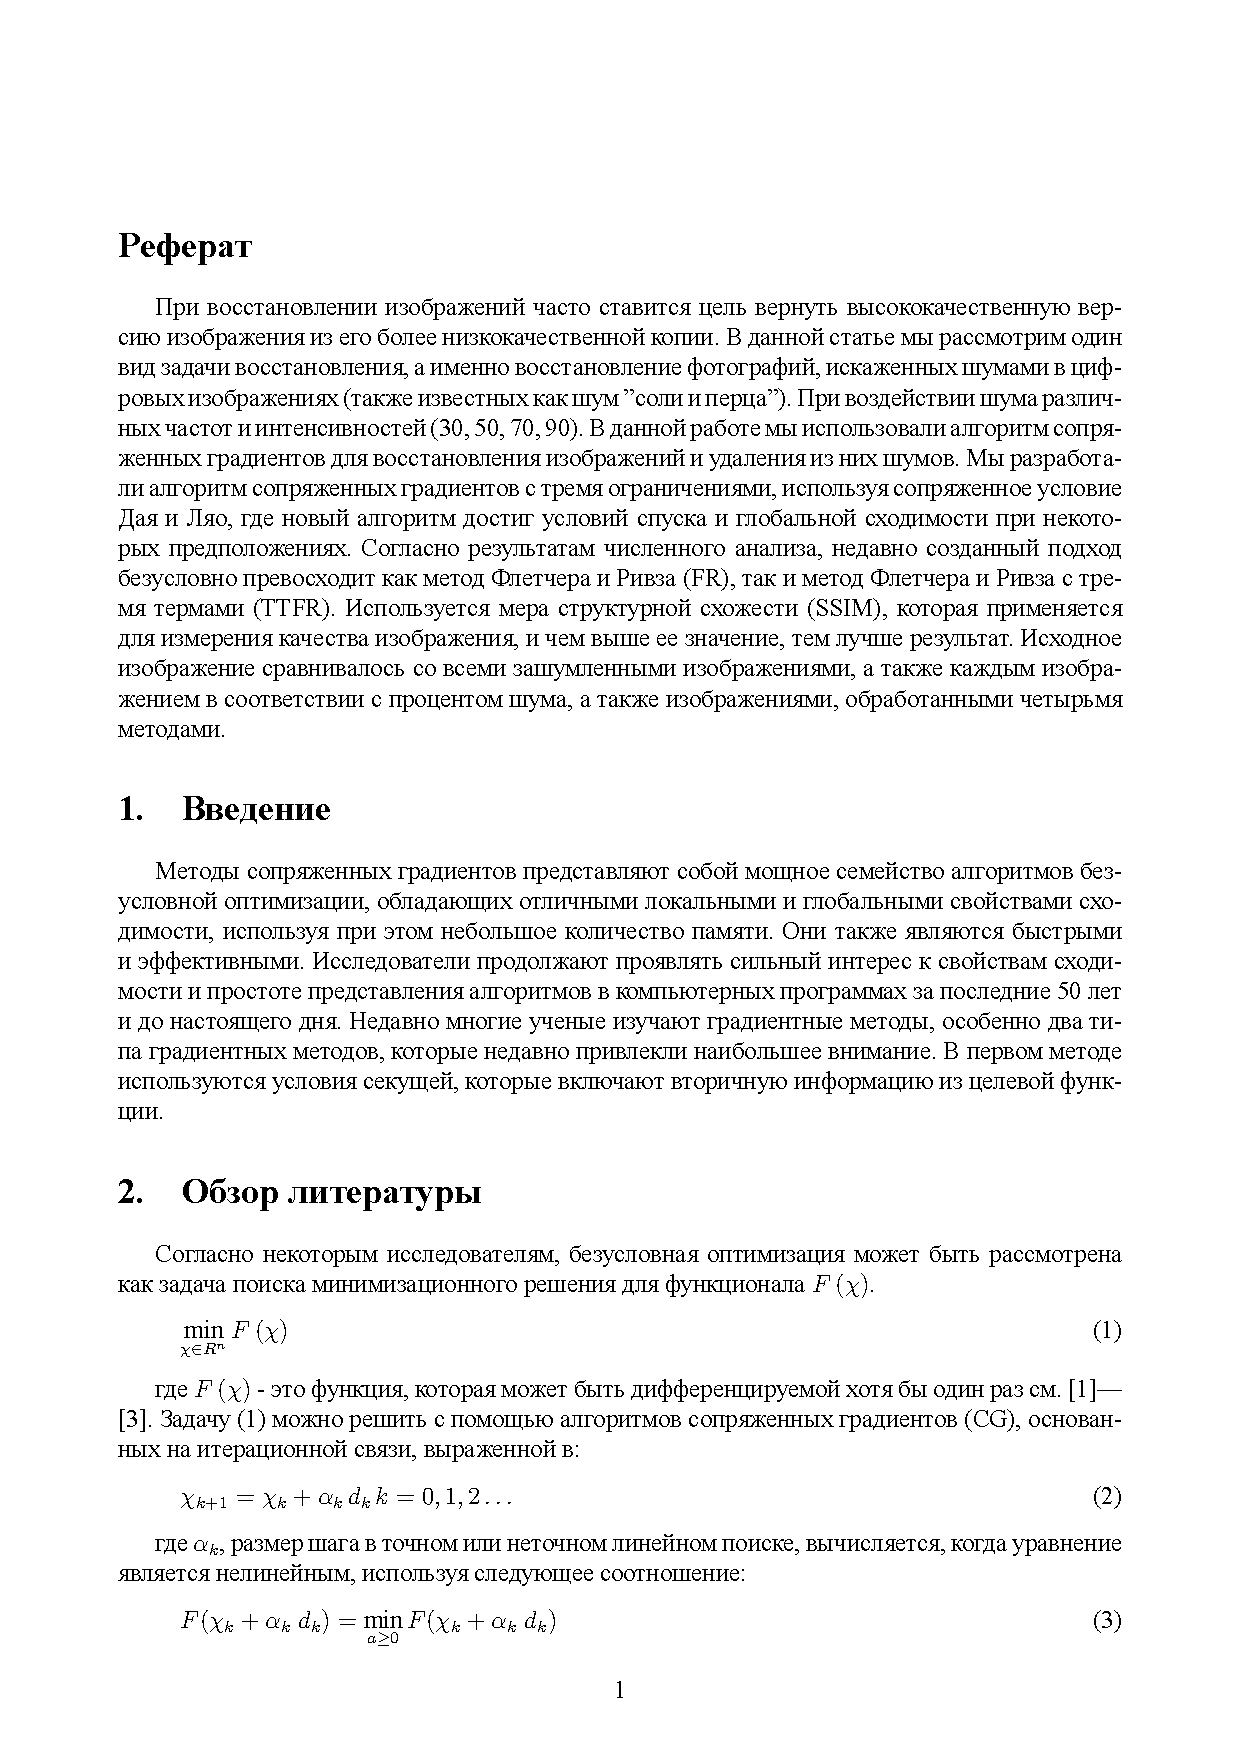
\includepdf[pages=1,offset=0 0, pagecommand={\subsection{Перевод статьи}\label{reference}\thispagestyle{plain}}
]{translation.pdf}

\includepdf[pages=2-,offset=0 0, pagecommand=\thispagestyle{plain}
]{translation.pdf}

\newpage
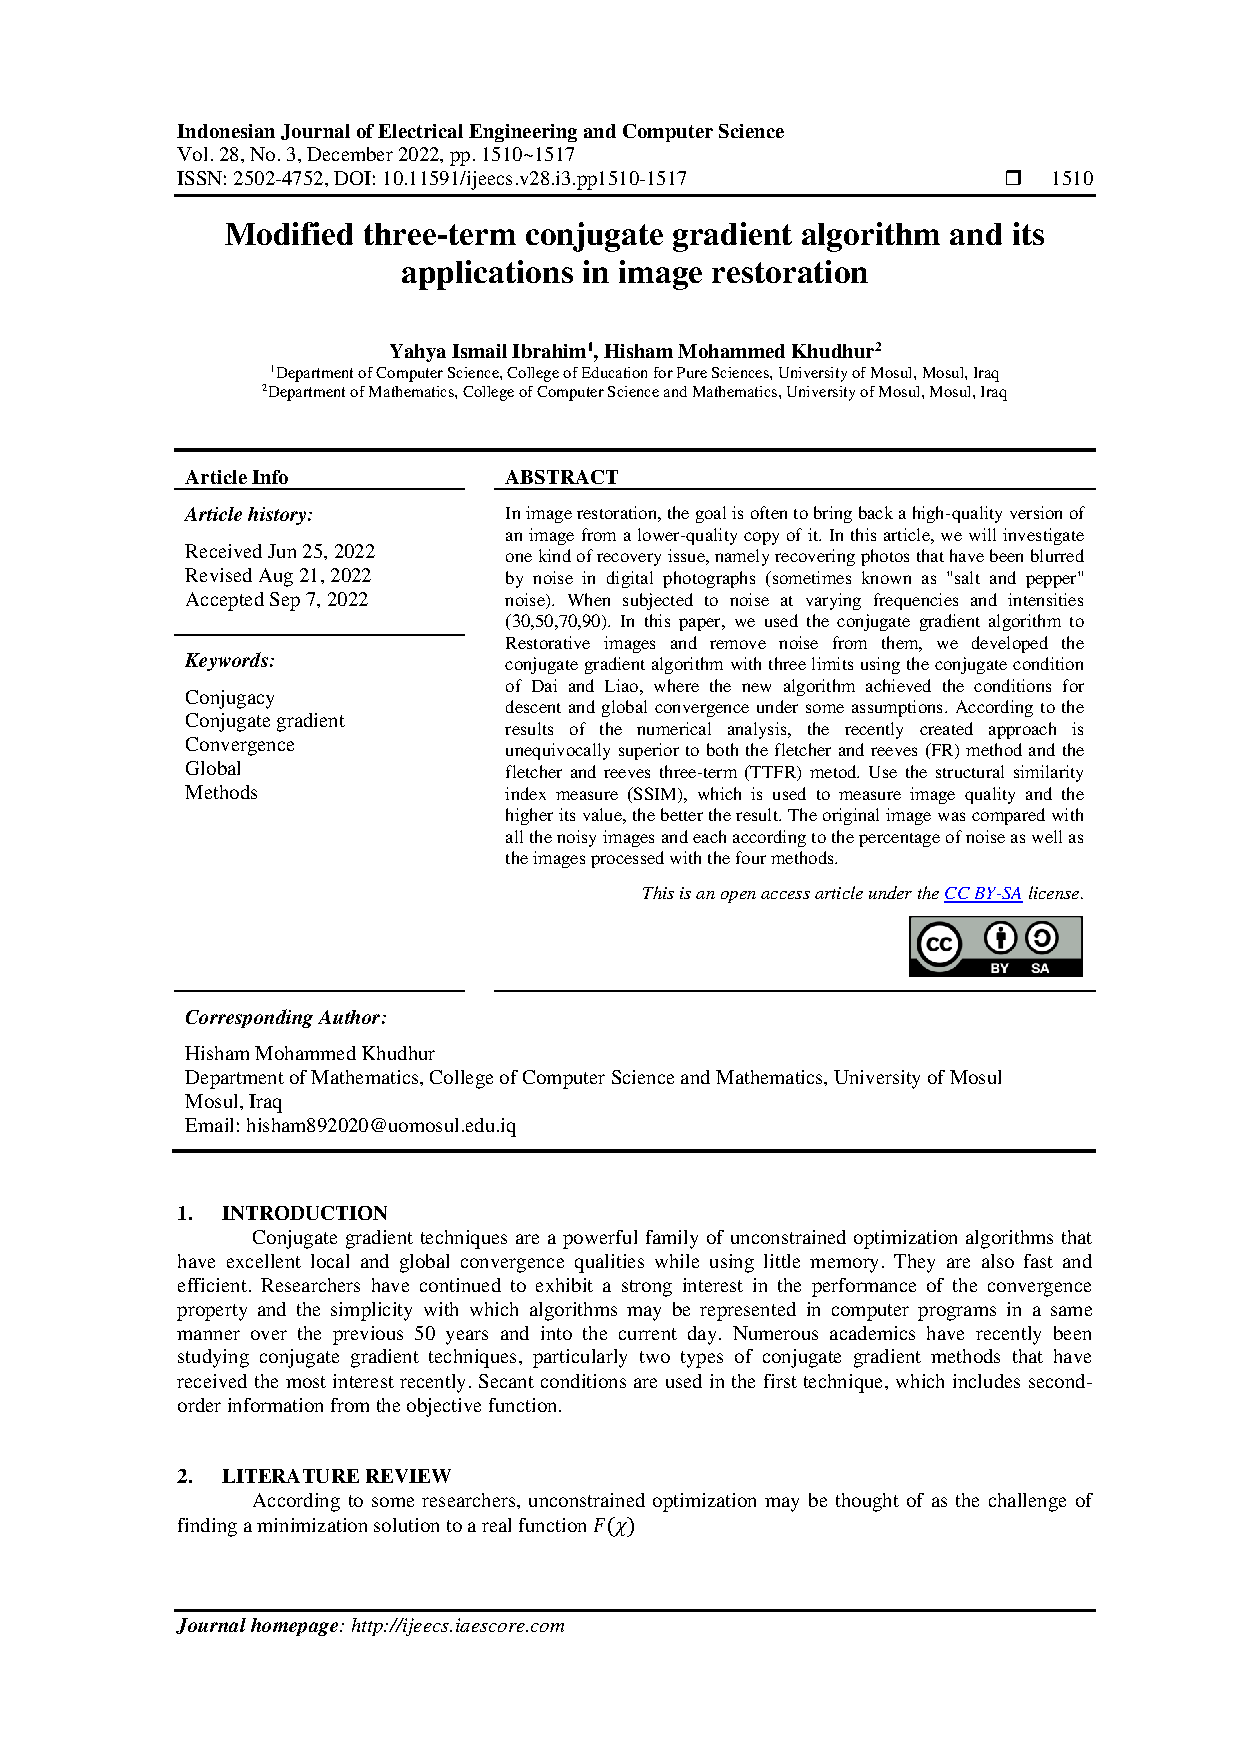
\includepdf[pages=1,offset=0 0, pagecommand={\subsection{Оригинальная статья}\label{reference}\thispagestyle{plain}}
]{Modified_three-term_conjugate_gradient_algorithm_a.pdf}

\includepdf[pages=2-,offset=0 0, pagecommand=\thispagestyle{plain}
]{Modified_three-term_conjugate_gradient_algorithm_a.pdf}

\end{document}
